%%%%%%%%%%%%%%%%%%%%%%%%%%  phdsymp_sample2e.tex %%%%%%%%%%%%%%%%%%%%%%%%%%%%%%
%% changes for phdsymp.cls marked with !PN
%% except all occ. of phdsymp.sty changed phdsymp.cls
%%%%%%%%%%                                                       %%%%%%%%%%%%%
%%%%%%%%%%    More information: see the header of phdsymp.cls   %%%%%%%%%%%%%
%%%%%%%%%%                                                       %%%%%%%%%%%%%
%%%%%%%%%%%%%%%%%%%%%%%%%%%%%%%%%%%%%%%%%%%%%%%%%%%%%%%%%%%%%%%%%%%%%%%%%%%%%%%


%\documentclass[10pt]{phdsymp} %!PN
%\documentclass[twocolumn]{phdsymp} %!PN
%\documentclass[12pt,draft]{phdsymp} %!PN
%\documentstyle[twocolumn]{phdsymp}
%\documentstyle[12pt,twoside,draft]{phdsymp}
%\documentstyle[9pt,twocolumn,technote,twoside]{phdsymp}
\documentclass[a4paper,oneside,12pt]{article}

\usepackage{pdfpages}
\usepackage{a4wide}
\usepackage[english]{babel} 
\usepackage{url}
\usepackage{caption}
\usepackage{multirow}
\usepackage{rotating}
\usepackage{soul}
 
\usepackage{palatino}

\usepackage{graphicx}
\graphicspath{{figures/}} 
\def\BibTeX{{\rm B\kern-.05em{\sc i\kern-.025em b}\kern-.08em
    T\kern-.1667em\lower.7ex\hbox{E}\kern-.125emX}}

\newtheorem{theorem}{Theorem}

% zet de paragrafen een beetje uit elkaar en links uitgelijnd
\setlength{\parindent}{0mm}
\setlength{\parskip}{1ex plus 0.5ex minus 0.2ex} 

\setlength{\textheight}{23cm}
\setlength{\textwidth}{16cm}
\setlength{\oddsidemargin}{0cm}
\setlength{\evensidemargin}{0cm}
\setlength{\topmargin}{-1cm}

\penalty-10000
\tolerance=10000

% \setlength{\parskip}{0pt}
% \setlength{\parsep}{0pt}
% \setlength{\headsep}{0pt}
% \setlength{\topskip}{0pt}
% \setlength{\topmargin}{0pt}
% \setlength{\topsep}{0pt}
% \setlength{\partopsep}{0pt}

\linespread{0.9725}

\usepackage[compact]{titlesec}
%\titlespacing{\section}{1pt}{*0}{*0}
%\titlespacing{\subsection}{1pt}{*0}{*0}
\titlespacing{\subsubsection}{1pt}{*0}{*0}

\usepackage{mdwlist}

\begin{document}


%-------------------------------------------------------------------------------------------

\thispagestyle{empty}

\begin{center}
\mbox{}\\\vspace{5mm}
{\Large Application for China Scholarship Council Grant}\\ [45mm]
%
{\bf\Huge Hardware acceleration for\\
[3mm] FPGA CAD Tools} \\
\vspace{45mm}
\Large Yun Zhou \\
\vspace{2mm}
\small\texttt{zhouyun\_zy@foxmail.com} \\
\vspace{20mm}
\Large Advisor: ir.\ Elias Vansteenkiste \\
\small\texttt{Elias.Vansteenkiste@ugent.be} \\
\vspace{2mm}
\Large Promotor: prof.\ dr.\ ir.\ Dirk Stroobandt \\
\small\texttt{Dirk.Stroobandt@ugent.be} \\
\vspace{20mm}
\normalsize Ghent University, Belgium \\
\normalsize Department of Electronics and Information Systems\\
\normalsize Computer Systems Lab\\
\normalsize Hardware and Embedded Systems Group 
\end{center}

\newpage

\tableofcontents

\clearpage

\section{Problem Definition \hl{(1 page)}}
A Field Programmable Gate Array (FPGA) is an integrated circuit made up of a grid of programmable functional blocks embedded in a programmable interconnection network. An FPGA is used to accelerate any arbitrary logic function in the same way as Application Specific Integrated Circuits (ASICs), however the functionality of an FPGA is not fixed during the production process. The functionality can be changed by writing a different configuration to the configuration memory. This flexibility leads to a substantial reduction of the economic risk of developing hardware accelerators. It also explains the rise in the popularity of the FPGA~\cite{putnam2015reconfigurable}. Unfortunately the flexibility of the FPGA comes at a price.  Each time the application developer wants to test his design, the design has to be compiled to an FPGA configuration and this is a complex and time consuming process. Unfortunately the designer typically needs to compile his application numerous times to test if his/her design meets the constraints of the application. 

The main FPGA device manufacturers and the academic community have developed a chain of heuristics to solve the NP hard problems involved in the compilation.
The compilation/translation of a high-level description of the application to an FPGA configuration is typically divided in several steps. In each step NP hard problems have to be solved and heuristics were and are being developed to try to approximate an optimal solution. The most time-consuming steps are the placement and routing steps. They are the last steps at the backend of the tool flow. These steps have to performed to obtain accurate timing information, which is needed to assess if the design meets the constraints. 
 
Another trend is the increase in both the size of applications and the size of the target devices. FPGA device and application sizes are still increasing following Moore's law~\cite{shannon2015technology}. Unfortunately the power of the FPGA CAD tools lags behind. The traditional CAD heuristics scale very badly in terms of application and device size, which translates to waiting times of hours up until days for compilation to finish \cite{murray2015timing}. 

Since the introduction of high-level synthesis~\cite{autoesl}, more and more engineers with a software background attempt to accelerate applications with an FPGA. They are used to gcc-like compilation times. Their design methodologies are adapted to these short compilation times. In order to fix bugs and measure performance the compilation is performed numerous times. Hence, they cannot accept the long compilation times that are common in FPGA design.

To overcome this problem, device manufacturers and academics developed multi-threaded versions of the heuristic algorithms \cite{ludwin2011,gort2012,betz2013method,jain2014multi}, but unfortunately scalability issues still exist and large designs still need hours to be compiled. To further speed up compilation a straightforward path is to use hardware acceleration, but unfortunately the current multi-threaded algorithms for placement and routing are hard to adapt for the wide scale parallelisation used in hardware accelerators such as GPUs and FPGAs.

Summary: \emph{FPGA design compilation takes too much time to allow efficient design turnaround times. Hardware acceleration of the compilation process is needed but the current placement and routing algorithms are not very well suited for this.
%Dynamische FPGA-herconfiguratie biedt vele voordelen. Op dit moment kan enkel de functionaliteit, maar nog niet het interconnectienetwerk van de FPGA gespecialiseerd worden op een automatische manier. Dit leidt tot veel manueel werk op het architecturaal niveau en dus heel dure en niet-herbruikbare implementaties.
} 

\newpage

\section{Goal \hl{(1 page)}}

\emph{In this Ph.D.\ research proposal, our aim is to significantly reduce the FPGA design compilation time by efficiently parallelizing placement and routing algorithms. In a first phase, we will parallelize and improve the existing placement and routing algorithm implementations. For the routing problem, we envisage that the existing routing algorithms will not allow a significant enough efficiency increase. Therefore, in a second phase, we will investigate new routing algorithms that are much more susceptible to parallelization and are much more efficiently accelerated by hardware than the current implementations.}

The overall high level goal is to reduce the FPGA design compilation time, but in this proposal we mainly want to focus on placement and routing, because they are the main runtime consumers \cite{vansteenkiste2015analyzing}. 


\hl{
prove
analyse
test
examine
}

In the proposal we want to investigate how much placement and routing can be accelerated by writing a specific GPU-kernel based on a massively parallelizable placement algorithm.
Our first aim is to have a modified version of the placement algorithm {\sc Liquid} that can be implemented on GPU. {\sc Liquid} is a placement algorithm that is being developed at Ghent University \cite{liquid}.  The second aim is to implement the adapted version of {\sc Liquid} with CUDA \cite{nickolls2008scalable} and demonstrate and measure its performance.

The next goal is to develop a new routing algorithm that is suitable for GPU Acceleration. Current graph based algorithms such as the omnipresent Pathfinder algorithm~\cite{} are not suited for wide-scale parallelism. We will investigate the introduction of new routing algorithms that are much more prone to exploiting massive parallelism for being accelerated by a GPU
implementation. Another option is to use an FPGA to accelerate the routing algorithm. In both cases, significantly novel routing techniques will have to be developed to enable a significant efficiency increase of the routing algorithm implementation.


\hl{Restrictions of the GPU}



\newpage

\section{Background \hl{(4 pages)}}
\label{background}
\hl{What is already known or unknown? Set the scene.}
\subsection{FPGA Architecture}
FPGAs are becoming ubiquitous components in digital systems and datacenters \cite{ovtcharov2015accelerating,putnam2015reconfigurable}. Their flexibility is one of the main reasons of the rise in their popularity. An FPGA can implement any arbitrary digital circuit. The only restriction is the size of the FPGA. To make this possilbe the FPGA is built up by an array of logic blocks. Each logic block contains several Look-Up Tables (LUTs) and Flip-flops (FFs). Each LUT is able to implement any boolean function of its inputs. To achieve this the truth table of the boolean function is written to the configuration memory of the LUT. The logic blocks are embedded in an interconnection network. The interconnection network can be configured by writing values to the memory cells for the switches.

\begin{figure}[t]
\centering
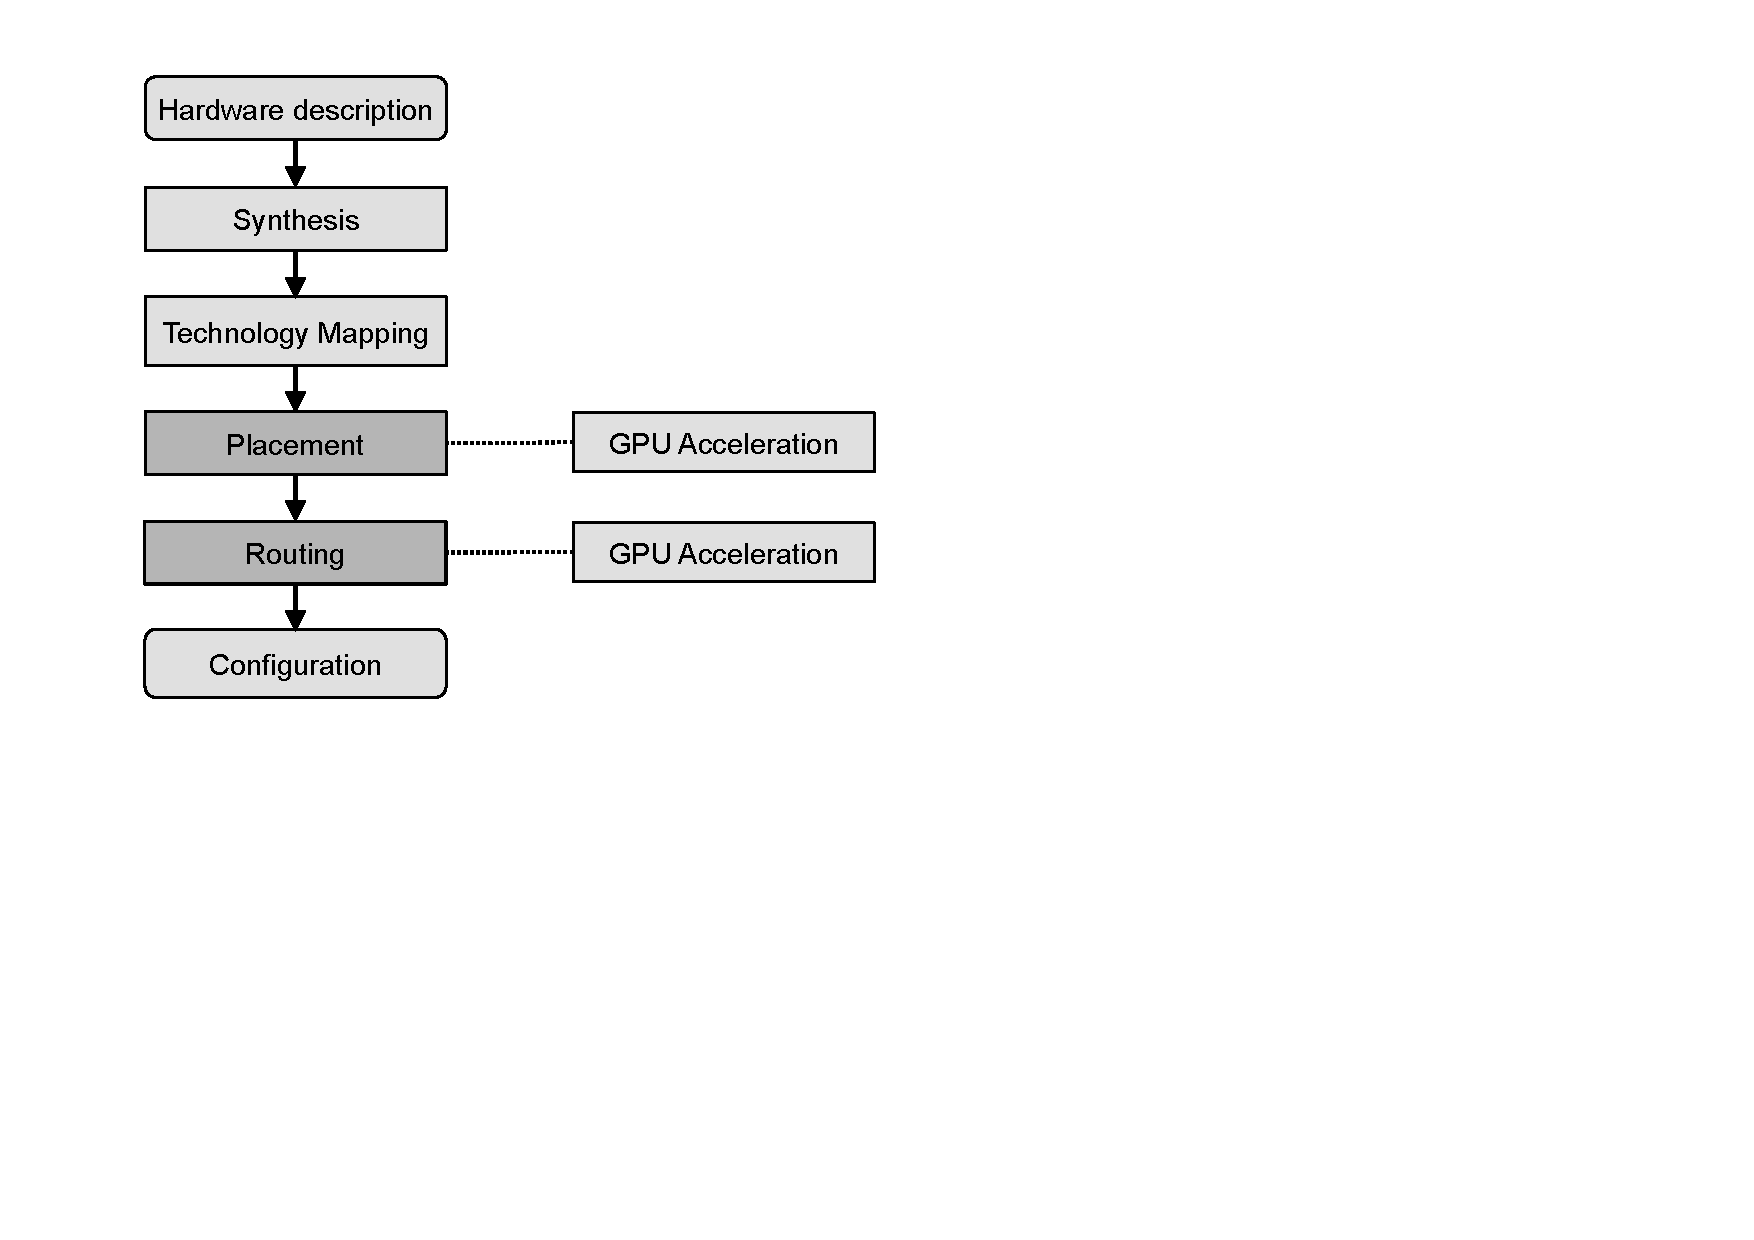
\includegraphics[width = 0.50\textwidth,trim = 0mm 90mm 140mm 2mm, clip]{toolflow}
\caption{Schematic representation of the toolflow. The placement and routing step will be accelerated by a GPU kernel.}
\label{toolflow}
\end{figure}

\subsection{The FPGA CAD tool flow}

An FPGA is configured at boot time by writing a bitstream to the configuration memory. Generating the bitstream is a complex task. Automatic tool flows are developed to aid the designer. These tool flows compile a bitstream starting from a high level description. To manage the complexity, the task is divided and dealt with by seperate tools. An overview of the toolflow is given in Figure \ref{toolflow}. 

\paragraph{Synthesis}
The designer describes the digital system in a high level description language (HDL) such as VHDL or Verilog or in a high level language such as SystemVerilog or OpenCL. In the synthesis step the description is translated to a netlist of logic gates, hard block instances, inputs and outputs.

\paragraph{Technology Mapping} 
The netlist of gates is mapped to a circuit with functional blocks present on the target device.

\paragraph{Placement}
The placer choses a block site on the FPGA for each functional block in the circuit and places the blocks according to the different optimisation goals. In order of increasing importance, the optimization goals are the total wirelength, routability and critical path delay. These goals are not independent. During placement the algorithm has to be able to estimate the quality of the placement at all times, therefore the optimization goals are estimated based only on the location of the functional blocks on the device. 

\paragraph{Routing} After placement the location of the functional blocks is known and enough information is available for routing the nets in the interconnection network of the target device. Routing a net can be reduced to  one of Karp's 21 well-known NP-complete problems, called Steiner Tree Problem. Additionally nets in a circuit can't share any routing resources, because this would lead to short-circuits. The router needs to find disjoint sets of routing resources, for each net one set. Most popular academic and commercial FPGA routers use a Pathfinder based algorithm~\cite{pathfinder, vprBVRJ, vprboek}.

\subsubsection{Runtime breakdown}
\begin{figure}[t]
\centering
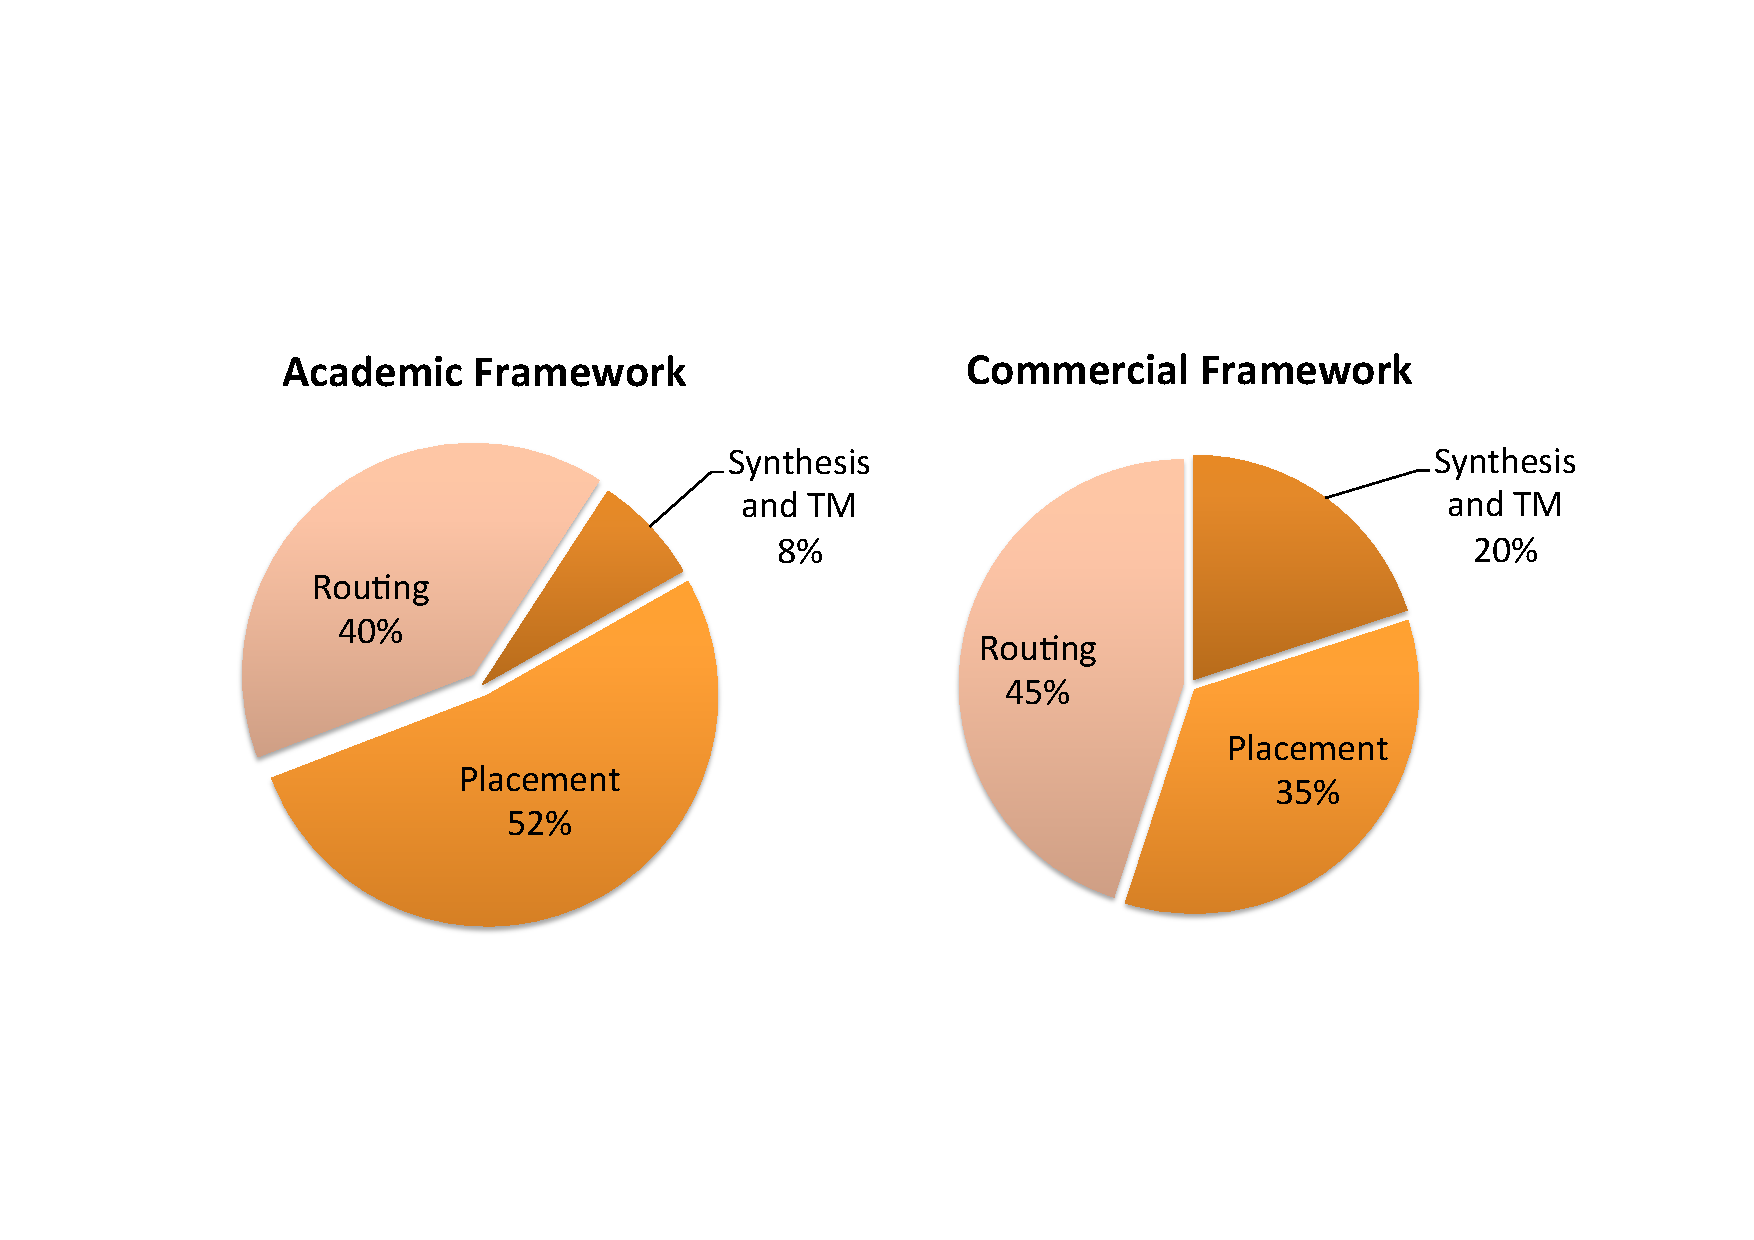
\includegraphics[width = 0.75\textwidth,trim = 0mm 50mm 0mm 40mm, clip]{runtime_breakdown}
\caption{Breakdown per tool of the compilation runtime.}
\label{rt}
\end{figure}

In Figure~\ref{rt}, a pie chart indicates the runtimes for the different steps in the compilation of the toolflow. These were obtained for the popular academic tool flow Verilog-To-Routing~\cite{luu2014vtr} and for the commercial tool flow from Xilinx, Vivado \cite{feist2012vivado}, using the framework in~\cite{vansteenkiste2015analyzing}. The majority of the runtime is clearly consumed by placement and routing. This is also stated by other important publications, such as \cite{murray2015timing}.

\subsection{Existing approaches \hl{(1.5 pages)}}

\subsubsection{The FPGA Placement Problem}
\label{sec:placeprob}
%The problem
An FPGA placement algorithm takes two inputs: the mapped input circuit and a description of the target FPGA architecture. The algorithm searches a legal placement for the functional blocks of the input circuit so that circuit wiring is optimised. In a legal placement every functional block is associated to (placed on) one of the physical blocks (without overlap) that is capable of implementing the functional block. 


%optimization goals
The main optimisation goal used by placement tools is to minimise the total wire length required to route the wires in the given placement. Placers that are only based on this goal are called wire-length-driven placers. More complex tools such as routability-driven \cite{swartz1998afrrff} and timing-driven placers \cite{marquardt2000tpff} trade some of the wire-length for
a more balanced wiring density across the FPGA or a higher maximum clock frequency of the circuit, respectively. 

%Dificult problem => Heuristic 
%Easy to addapt => Simulated annealing
Finding a high quality placement is very important, because poor  quality placements generally cannot be routed or lead to low operation frequencies and high power consumption. Worse, the placement problem is computationally hard, so there are no known algorithms that can find an optimal solution in a reasonable time. Therefore, many heuristics have been developed for the placement problem. Most of these algorithms belong to one of three types of placers: partition-based placers \cite{maidee2005tppfisf}, analytic placers \cite{chan2003ppffga} and simulated annealing placers \cite{betz1997vanppartffr}. 

%\todo{Is dat eigenlijk wel waar dat SA placers gemakkelijkst aan te passen zijn? Heb je daar ook argumenten voor. Je kan wel zeggen dat deze plaatser met een kostfunctie werkt en enkel die kostfunctie aangepast moet worden maar de anderen zijn misschien even gemakkelijk aan te passen.}

\subsubsection{Simulated Annealing}
Simulated annealing \cite{kirkpatrick1983obsa} is inspired on annealing of metals, a technique involving heating and controlled cooling of a material to increase the size of its crystals and reduce their defects.

\paragraph{The Basic Algorithm}\hl{I think here you can significantly shorten.}
At any time, the algorithm keeps track of the placement cost. In a wire-length-driven placer this is the sum of the estimated wire-lengths over all nets. The algorithm starts by randomly, but legally, placing the logic blocks in the input circuit on physical blocks of the FPGA architecture. Afterwards, the placer repeatedly tries to interchange the logic blocks placed on two randomly chosen physical blocks. Such an interchange is called a move. If the move causes a decrease in placement cost, the move is always accepted. If on the other hand, the move causes an increase in placement cost the move is accepted with a probability of $e^{-\frac{\Delta C}{T}}$, where $\Delta C$ is the change in cost due to the move and $T$ is a parameter called the temperature, which controls the probability by which hill-climbing moves are accepted. Initially, $T$ is very high so that most moves are accepted. Gradually $T$ is decreased so that the probability by which hill-climbing moves are accepted decreases. When the temperature is decreased in the proper way the result is a low cost placement. The hill-climbing moves allow the placer to escape from local minima.

The initial temperature, the rate at which the temperature is decreased, the number of moves that are attempted at each temperature, the way in which potential moves are selected and the exit criterion of the annealer are called the annealing schedule. A good annealing schedule is crucial for finding a good solution in a reasonable amount of time.

\paragraph{Wire-length Estimation}
\label{sec:wireLengthEstimation} The only way to exactly calculate the total wire-length of a given placement is to route the wires in a placement and sum the wire-length over all nets. Since routing is in itself a computationally hard problem, solving it repeatedly for every move tried in the inner loop of the placer and in this way exactly calculating the total wire-length, leads to very long execution times for the placer. Therefore, the cost is not exactly calculated but estimated.

A common way of estimating is calculating the sum of the estimated wire lengths of each net, where the wire length of a net is estimated as the half-perimeter of its bounding box weighted by a factor which depends on the number of terminals of the net (taken from \cite{cheng1994raaeprm}). %It is equal to 1 for nets with up to three terminals and slowly grows to 2.79 for nets with 50 terminals.

\paragraph{Problems with using Simulated Annealing}
Typically the number of moves performed per temperature step is not linear with the number of blocks, which leads to long runtimes.
Although it seems straightforward to adapt simulated annealing for multiple threads, the quality of the solution and the speedup gain per thread deteriorate fast as the number of threads increase \cite{ludwin2011}. This is mainly caused by collisions and synchronization issues. In multi-threaded solutions each thread swaps blocks independently, instead of swapping blocks sequentially.

\subsubsection{Analytical Placement}
In analytical placement the placement problem is represented as a linear system of equations. Solving this linear system gives us the optimal locations for the blocks in the circuit. The system of equations is obtained by taking the partial derivatives of the square of the total wire-length. 
% in order to minimise the wire length. 
Unfortunately the solution typically does not contain discrete block positions and blocks may overlap. However, placing blocks on the FPGA requires blocks to not overlap and the block positions are located at discrete positions. 
To overcome this the solution is legalised, but after legalising we typically end up with a detoriated placement. To improve the placement, a new system of equations is built not only based on the wire length of the connections, but also on the distance to the legalized position, called anchor positions. These anchors are refreshed each time a solution is legalized.
Multiple iterations of solve-legalize are performed, while increasing the weight of the anchor connections. The algorithm typically stops if the decrease in cost of the legalized solution starts to slow down and converge towards the cost of the solved solution.  The solution typically converges after 20 iterations, depending on how fast anchor weights are increased. 

\paragraph{Problems with using Analytical Placement}
Each iteration the linear system is solved, it takes time to build it. A matrix of size NxN is to be constructed, with N being the number of connections. Although the matrix is sparse and can be stored efficiently with compressed row format, it requires extra memory, making analytical placement less scalable in terms of memory.
Both solving the linear system and the legalisation method are hard to parallelise and require synchronisation.

\subsubsection{The FPGA Routing Problem}
Once the placement algorithm has placed each of the logic blocks of the input circuit on a physical block of the FPGA architecture, the router needs to determine which of the switches in the routing architecture need to be closed and which need to be opened in order to connect the physical blocks in accordance to the way their associated logic blocks are connected in the input circuit. The goal is not only to find a legal routing solution but also to try to maximise the circuit clock frequency by allowing critical paths to use shorter and faster routing resources.

\paragraph{Routing-resource Graph}
{\sc pathfinder} \cite{mcmurchie1995panprff} uses a directed graph, called the {\em Resource Graph}, as a model for the routing architecture of an FPGA.  Because this graph can be constructed for any useful routing architecture, the algorithm is very flexible. 

The resource graph is a directed graph $C=(N,E)$, where the nodes $N$ represent the routing resources. A directed edge $(t,h)$ represents the possibility of routing a signal from resource $t$ (the tail of the edge) to resource $h$ (the head of the edge), by setting a switch. There are five types of routing resources: wire segments, input pins, output pins, sinks and sources. Unidirectional switches which, when closed, force the logic value of resource $i$ on resource $o$, are modeled as a directed edge $(i,o)$.

When the routing architecture of the FPGA is represented as a routing-resource graph, the routing algorithm reduces to finding a subgraph of the routing-resource graph, called a routing tree, for each of the nets. These routing trees should be disjoint to avoid short circuits. Each routing tree should contain at least the source nodes and the sink nodes of its associated net and enough wire nodes so that a connection exists between the source node and each of the sink nodes.

\subsubsection{{\sc Pathfinder}: A Negotiated Congestion Router}
\label{sec:pathfinder}
The {\sc Pathfinder} algorithm \cite{pathfinder} tries to solve the problem in several iterations. In every routing iteration, the algorithm rips up and reroutes all the nets in the input circuit. These iterations are repeated until no shared resources exist \cite{nair1987asyetfgw} or, in other words, the routing trees of the nets are disjoint. This is achieved by gradually increasing the cost of sharing resources between nets. During the first iteration, nets can share resources at no extra cost and thus, each net is routed with a minimum number of wires. The cost of a routing resource does not only depend on the current sharing cost but also on the sharing history of the resource. Resources that were shared heavily in past routing iterations become more expensive. In this way a congestion map is built, which enables nets to avoid routing through heavily congested resources, if possible.

\paragraph{Routing a Net}
The task of the net router is to find a minimum cost routing tree for a given net in the resource graph. As mentioned before, the routing tree should contain the source and the sinks of the net and a path from the source to each of the sinks. The cost of the resources is determined by the negotiated congestion mechanism.

The search space of all possible routing trees for a net is huge. Therefore a heuristic was developed that finds a low cost routing tree for a given net in a reasonable amount of time. Typically a variant of a maze router is used~\cite{lee1961aafpcaia}. The maze router loops over all the sinks of the net and extends the already found routing tree with the shortest path from this routing tree to the sink under consideration. The shortest path is found using Dijkstra's algorithm \cite{dijkstra1959anotpicwg}.

\begin{figure}[ht]
\centering
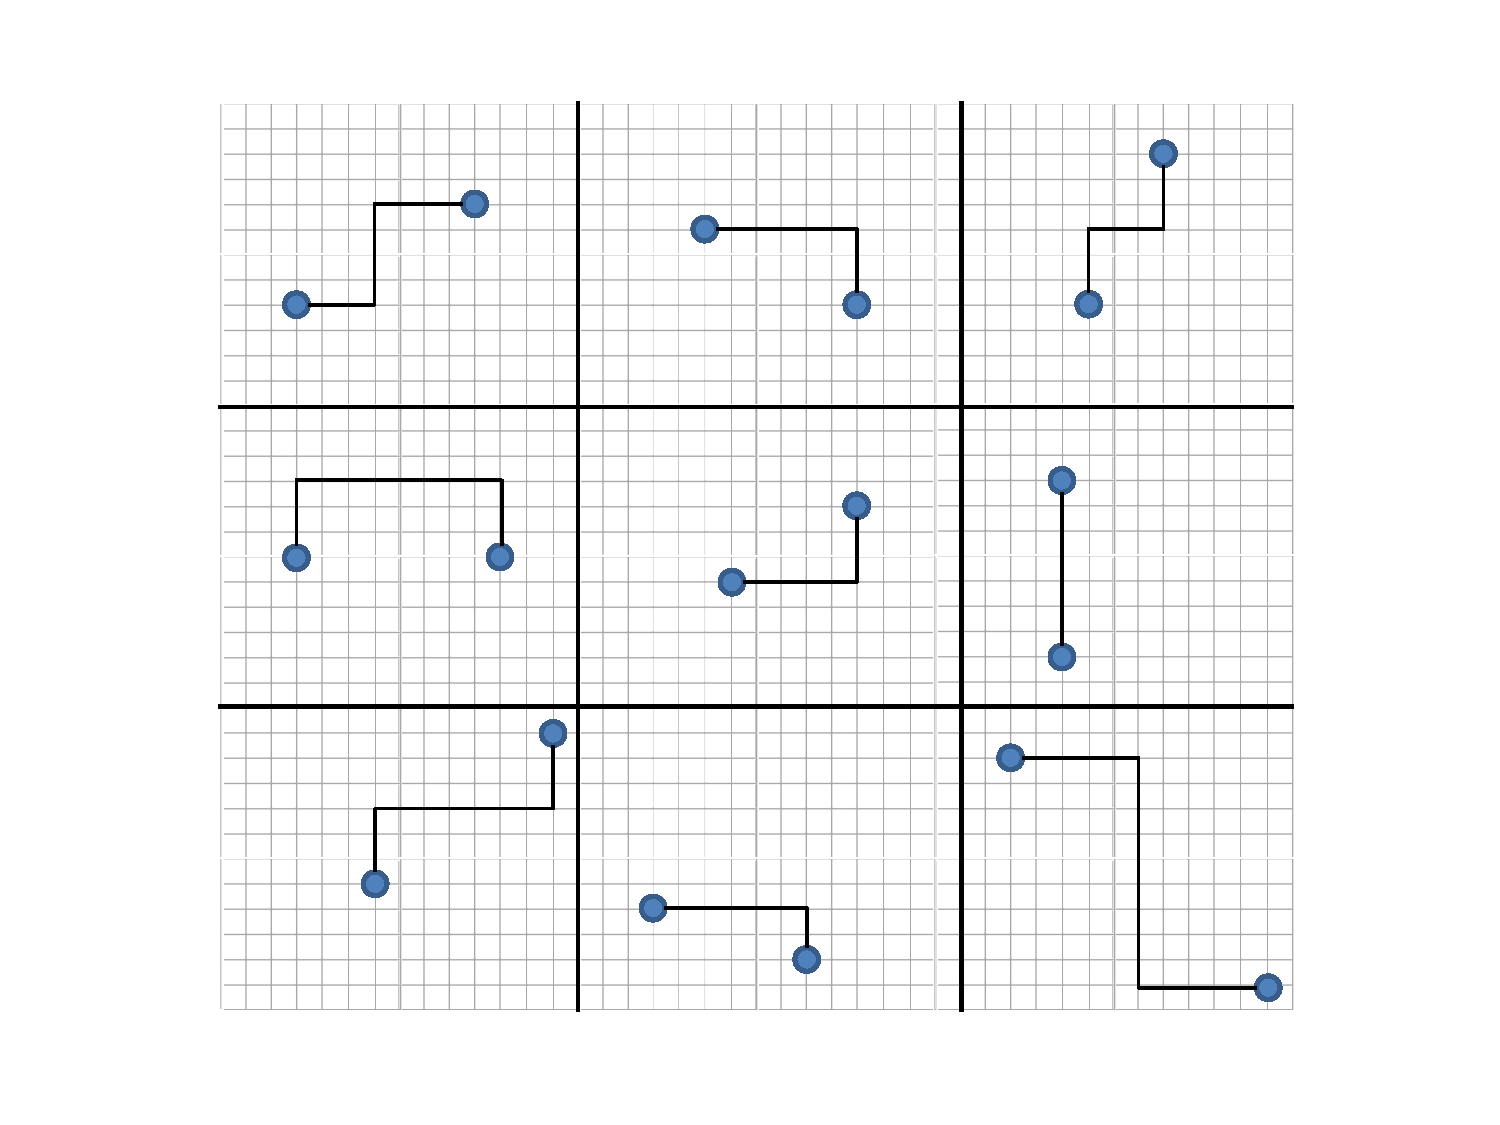
\includegraphics[width = 0.4\textwidth,trim = 0mm 0mm 0mm 0mm, clip]{parallellisatie}
\caption{Breaking up sets of nets based on the location of their terminals.}
\label{geopara}
\end{figure}

\subsubsection{State-of-the-art advances in routing techniques}
In~\cite{vansteenkiste2013connection} the authors were able to further refine the negotiated congestion mechanism to the level of connections. Nets are partially ripped up and rerouted, this allows us to only reroute congested connections, which helps us to avoid large routing runtimes for the large fanout nets. Others have developed multi-threaded routers. Gort et al. developed a multi-threaded router that splits up the nets in a circuit depending on the location of their terminals on the FPGA~\cite{gort2010deterministic}. Two nets can be routed concurrently in case they have terminals that are not located in each others bound box, as depicted in Figure~\ref{geopara}.
Another advance is the dynamic expansion of the routing resource graph, which leads to a reduction in memory usage~\cite{moctar2015fast}. 	
Adapting the routing architecture to speed up the routing is what the authors tried in~\cite{gort2013combined}.


\section{My research \hl{(2.5 pages)}}

\subsection{Placement techniques}\label{placetech}

For placement we have a clear proposal, because the research group HES, that I would be part of, has developed a placement algorithm with large scale parallelism in mind. The algorithm is called {\sc Liquid} and a single threaded version is available~\cite{liquid}.

\paragraph{{\sc Liquid}}
{\sc Liquid} is based on analytical placement. It is also an iterative algorithm in which optimised placement and legalised versions of the placement are generated in each iteration. In contrast to analytical placement there is no linear system that is solved in each iteration. In each iteration all the blocks are moved a few times.  The blocks are moved in the direction of the steepest gradient descent. For each block a move vector is calculated based on the previous position of the other blocks that are attached to it. The cost function is the sum of the estimated routing and timing cost of the nets attached to the block. All movement vectors can be calculated independently, which makes it uniquely suitable for parallelisation.

%texture with all positions of previous locations

\paragraph{Legalizer}
In the current implementation the blocks are moved following the steepest gradient descent a few times before the positions are legalised. The legaliser tries to spread, the blocks and assign a legal position to each block without any overlapping blocks. Regions of overlapping blocks are gradually spread, but sometimes two regions clash while expanding the region. This and similar edge cases have to be captured and handled correctly. This is hard to make concurrent, because there are a lot of dependencies between the blocks. 
Instead, our idea is to keep the movement of the blocks independent and introduce a legalising phase in which we will move the blocks a few steps not following the steepest gradient descent of the cost function, but trying to move each block to a legal position, while also repelling each other to prevent overlap. These moves will not lead to a completely legalised solution, but a nearly legalised solution. Based on experiments we know that it does not really influence the quality of the final solution if the intermediate solutions are not completely legalised.  At the end there will be one step of completely legalising, but this will be performed on the CPUs.

\paragraph{Timing analysis}
In a timing analysis the most critical connections are identified by traversing the timing graph. The connections determine the weights of the nets.
In the current implementation of {\sc Liquid}, we don't do a timing analysis after each optimize-legalise iteration, but we only do it each 5 iterations, because the criticality of the nets doesn't change extremely between iterations. 
So there is an option to do timing analysis on the CPUs concurrently, while the moves are being performed by the GPUs, but it will be the subject of research if this will degrade the quality of result of the final placement.
Another research path will be to also adapt timing analysis to be able to run it on the GPU. This will involve accelerating breadth-first search, because that is one of the main components of timing analysis. This is not straightforward because it involves graph traversal and pointer chasing, but Merrill et al. showed significant speedups in \cite{Merrill2015}.






\subsection{Routing techniques}\label{routetech}

Many multithreading strategies for the routing problem have been proposed in the past, but the limitations of the SIMD architecture present in GPUs forces us to simplify the problem if we want to make use of the massive parallelism offered by the GPU.
In what follows we describe the different strategies that will be investigated during the Ph.D.\ research. Depending on the feasibility, different strategies may be combined.

\paragraph{Route sets of connections in parallel} 
As mentioned in Section~\ref{background}, the first routing iteration takes the largest portion of runtime because each connection needs to be routed.
Important is that the connections in the first iterations are routed independently because in the first iteration the router typically does not take into account congestion cost, but only delay. Routing the connections can be done in parallel. Routing a connection is done by performing an A*-search in the routing resource graph of the FPGA.
The A* path-finding search algorithm is very famous in games for finding the shortest distance between two nodes. Today's games have thousands of agents moving at the same time in a cost field. Thus it has become very important to find shortest paths concurrently and in a speedy way. Making use of GPU's highly parallel multi-threaded nature suits this scenario perfectly \cite{bleiweiss2008gpu,bleiweiss2012system}.
 All A*-search wavefronts will be started in parallel. Each thread will behave as a single router. It will have its own priority queue. The instructions will be the same for all router threads and can therefor be executed in one warp. Pop a node from the priority queue. Check if we reached our target and if not add the neighbours to the priority queue. After each router thread found its target, a new warp can be started with threads that backtrace the path that lead to the target. Each thread spawns its own routing trace on a per cycle basis. For each connection there will be one backtrace thread. All backtrace threads will have the same instructions. They are also responsible for producing a series of history congestion cost updates. These updates are used after a batch of connections is done to build/update the congestion map.
% foreseeable problem: investigate visitation statuses of the nodes in the graph

\paragraph{Parallelize the Search}
A finer grained approach is parallelizing the A*-search in itself. The wavefront is expanded by different threads. A fixed number of nodes are popped from the priority queue and each thread processes the node separately. Each thread checks if the target is reached and if not the cost of the neighbouring nodes is calculated and added to the priority queue in a similar way as done in~\cite{Merrill2015}. The wavefront of an A*-search is typically directed towards the goal and so it only makes sense to expand a limited amount of nodes at a time, so we suggest to use the maximum number of threads in one warp, this is typically 32. This finer grained approach could be applied in the later router iterations in which the negotiated congestion mechanism is more sensitive to synchronization and connections have to be routed one after the other or only connections in other locations can be routed concurrently~\cite{gort2010deterministic}.

\paragraph{Tile based Compression of the Routing Resource Graph}
The routing resource graph (RRG) is actually built up of stitched instances of a few regular tiles. An expanded RRG can easily surpass today's workstation memory capacities \cite{murray2015timing}. It is important the routing resource graph fits in the GPU memory banks.
An FPGA consists of a grid of logic blocks interspersed with columns of memory blocks and DSP blocks. The interconnection fabric surrounding each type of block is typically adapted to the size and the number of I/O of the block. For each tile type a template RRG tile can be kept in the shared memory of the router threads. It is constant and read-only.
Tile-based compression of the RRG has been attempted in the past \cite{chin2007memory}, but was only evaluated in a single thread implementation on a CPU.

%Elias -> Dirk: In case you have any ideas about this let me know or you could write something up by yourself.
%\paragraph{Move away from graph based routers}
% Routing resource graph
%graph based
%move away from graph based routing algorithms

\newpage

\section{Timetable \hl{(1 page)}}\label{timetable}
\hl{ Indicate the timeframe for each broad stage considering literature surveys, data collection, production, modelling, review, analysis,
testing, reporting, chapter and thesis writing, and thesis submission date.}

The research in this project will be divided in 2 big stages:

%\subsection{Work Packages}
\begin{description*}
\item[Hardware Acceleration of the placement (24 months)]\ %(20 months)]\

\begin{description*}
\item[Adapt the {\sc Liquid} placement algorithm for wide-scale parallelization (9+1 months)]\
In the first step the placer prototype will be further developed and elaborated with the features that were described in the previous section. After this work there is one month allocated for writing a conference paper to report about the initial results.
\item[Implementation of GPU Accelerator for Placement (9+1 months)]\
\\After developing the placement algorithm, it will be implemented on the GPU. Measurements and results will be reported in another conference paper and a demonstration will be held at one of the workshops accompanying a conference. 
\item[Explore the concurrent execution of timing analysis (3+1 months)]\
While the GPU implementation is calculating the moves, the timing analysis can be performed concurrently on the CPU. If this does not degrade the quality of the result, we will also publish a paper on this. In the other case, we will try to accelerate timing analysis on the GPU as well.
\end{description*}

\item[Hardware Acceleration of the routing (18 months)]\

\begin{description*}
\item[Exploration of new routing algorithms for wide-scale parallelization (8+1 months)] 
Exploring different routing algorithms and devising new algorithms with wide-scale parallelisation in mind. After exploration, the prototype will be implemented and tested. The results will be reported in a conference publication.
\item[Implementation of GPU/FPGA accelerator for Routing (8+1 months)]
After developing the routing algorithm, it will be implemented on the GPU/FPGA. Measurements and results will be reported in another conference paper and a demonstration will be held at one of the workshops accompanying a conference. 
\end{description*}

\item[Writing the doctoral thesis and reporting final results (6 months)] This time is allocated to write the thesis and to report the finalized results in journals and conferences.  

\end{description*}

\begin{figure}[ht]
\centering
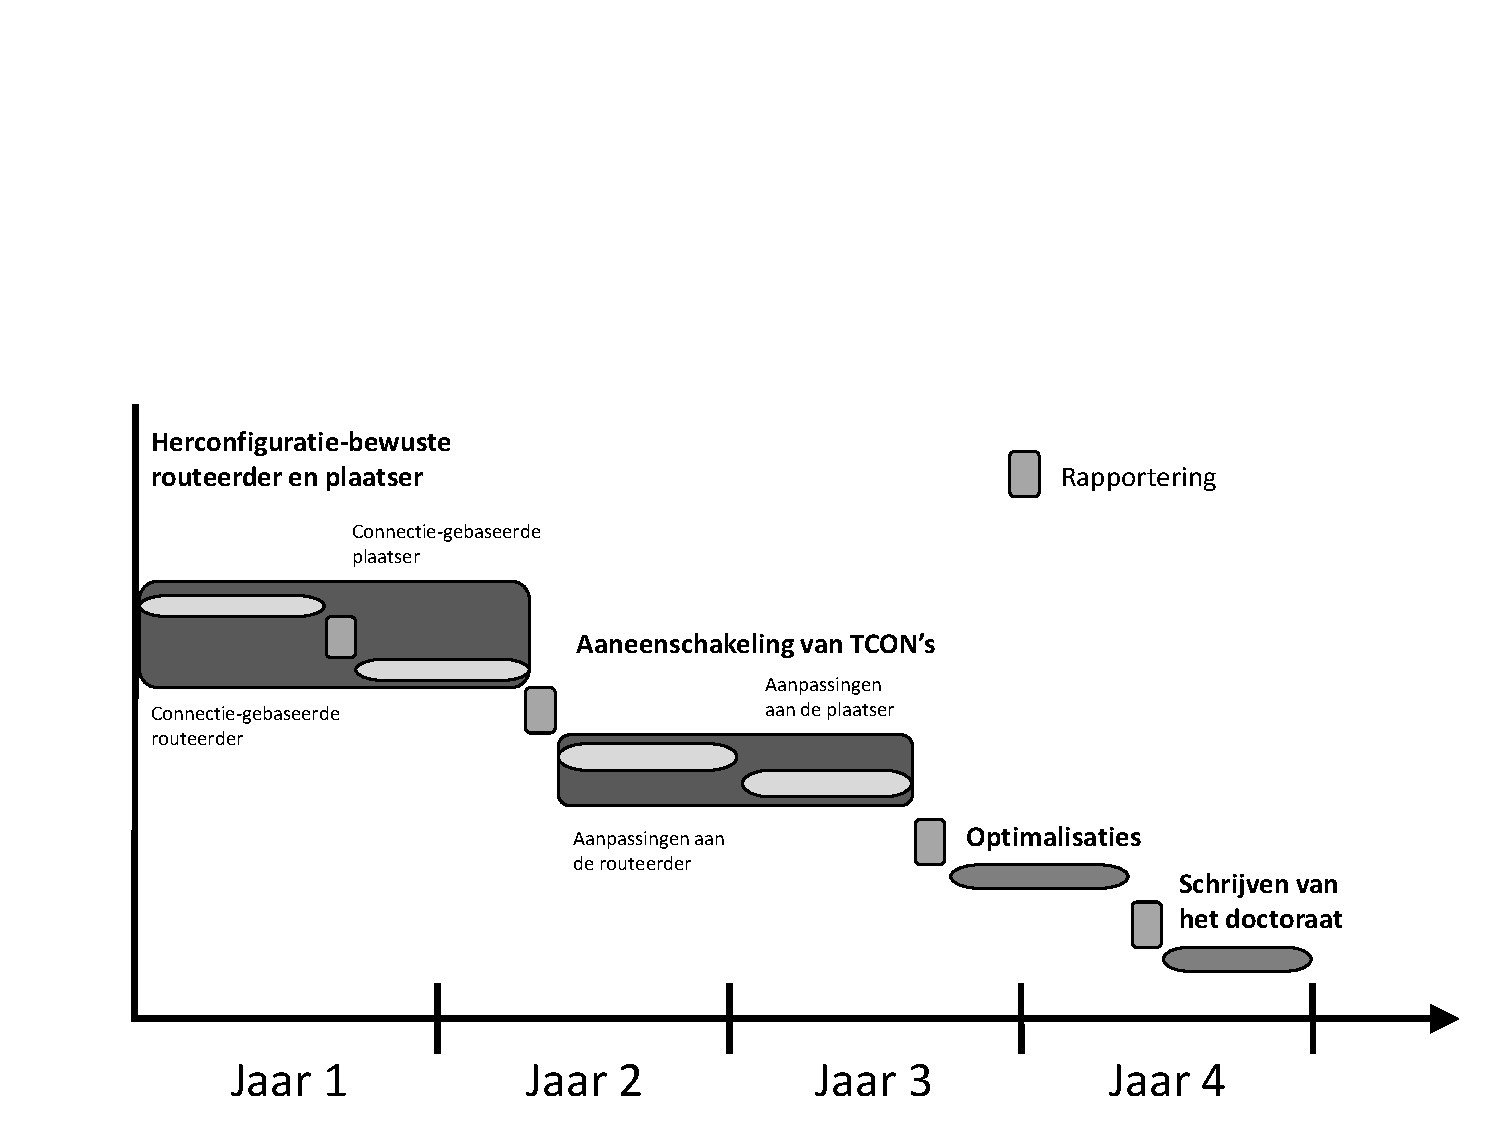
\includegraphics[width = \textwidth,trim = 0mm 0mm 0mm 70mm, clip]{tijdschema.pdf}
\end{figure}

\newpage
\section{Feasibility\hl{(1 page)}}
\hl{Expected outcomes, significance or rationale
Why is it important? 
What do you expect it will deliver? 
What are the expected outcomes? 
Establish the importance of your project by highlighting its originality or why it is worth pursuing. Highlight the benefits, positive expected outcomes or innovative applications of knowledge.}

\hl{@Yun: Can you make/update the figure for the planning/timetable?}

\subsection{Expected Outcomes}
The acceleration of placement and routing tools by parallelization and implementation of the algorithms on GPU or FPGA hardware will significantly shorten the design cycle for FPGA designs. This enables a strong reduction of the FPGA design turnaround time and hence speeds up the optimization of FPGA designs. The results of this project will therefore benefit thousands of designers worldwide.

Researchers have tried to parallelize placement and routing algorithms before but the benefits have not been tremendous because previous research has mainly focused on the simulated annealing based placers which are very difficult to parallelize. The prospects for parallelization of the analytical placement tool {\sc Liquid}, developed at Ghent University, are much better. Therefore, we are confident that we will succeed in obtaining very large speed-ups in the placement step (in part I of this research project). Although the reduction of time needed for placement alone already will prove significant, our goal is to go for the additional speedup of also parallelizing the routing step of the FPGA design cycle (part II of this research project). Although more challenging, we believe that the lessons learned from the parallelization of the placement step will help us in finding requirements for a new routing algorithm that is much better suited for parallelization. 

\subsection{Context and Strategy}\label{context}
This research will be conducted at Ghent University in the research group Hardware and Embedded Systems (HES). HES is part of the Computer Systems Lab (CSL) in the Department of Electronics and Information Systems. The HES group is lead by professor Dirk Stroobandt. The group has a lot of experience with developping FPGA CAD tool software and has developed the {\sc Liquid} analytical placer. The group also has worked a lot on improving routing tools (mainly to extend them in the context of run-time reconfigurable routing). It is the strategy of the group to further its expertise in placement and routing algorithms, as well as exploit its knowledge on hardware implementations for accelerating algorithms. The group's extensive contacts with the major researchers in the field worldwide and its active presence at the most important FPGA design conferences will further feed this project with ideas and suggestions and will help to keep it focused on its goals.



\newpage
%\nocite{*}
\bibliographystyle{phdsymp}
\bibliography{proposal} % commented if *.bbl file included, as
%\bibliography{../../../bib/hes} % commented if *.bbl file included, as
%%%%%see below
%%DIrk_bis: in je referenties hoofdletters escapen door ze tussen {} te zetten, zoals voor {FPGA}'s.

%%%%%%%%%%%%%%%%% BIBLIOGRAPHY IN THE LaTeX file !!!!! %%%%%%%%%%%%%%%%%%%%%%%%
%% This is nothing else than the phdsymp_sample2e.bbl file that you would%%
%% obtain with BibTeX: you do not need to send around the *.bbl file        
%%
%%---------------------------------------------------------------------------%%
%
%\begin{thebibliography}{1}
%\bibitem{LaTeX}
%Leslie Lamport,
%\newblock {\em A Document Preparation System: \LaTeX, User's Guide and
%  Reference Manual},
%\newblock Addison Wesley Publishing Company, 1986.
%\bibitem{LaTeXD}
%Helmut Kopka,
%\newblock {\em \LaTeX, eine Einf\"uhrung},
%\newblock Addison-Wesley, 1989.
%\bibitem{TeX}
%D.K. Knuth,
%\newblock {\em The {\rm T\kern-.1667em\lower.7ex\hbox{E}\kern-.125emX}book},
%\newblock Addison-Wesley, 1989.
%\bibitem{METAFONT}
%D.E. Knuth,
%\newblock {\em The {\rm METAFONT}book},
%\newblock Addison Wesley Publishing Company, 1986.
%\end{thebibliography}
%
%%---------------------------------------------------------------------------%%

\end{document}

%%%%%%%%%%%%%%%%%%%%%  End of phdsymp_sample2e.tex  %%%%%%%%%%%%%%%%%%%%%%%%%%%

